%%%%%%%%%%%%%%%%%%%%%%%%%%%%%%%%%%%%%%%%%%%%%%%%%%%
%
%  New template code for TAMU Theses and Dissertations starting Fall 2012.
%  For more info about this template or the
%  TAMU LaTeX User's Group, see http://www.howdy.me/.
%
%  Author: Wendy Lynn Turner
%	 Version 1.0
%  Last updated 8/5/2012
%
%%%%%%%%%%%%%%%%%%%%%%%%%%%%%%%%%%%%%%%%%%%%%%%%%%%

%%%%%%%%%%%%%%%%%%%%%%%%%%%%%%%%%%%%%%%%%%%%%%%%%%%%%%%%%%%%%%%%%%%%%%%
%%%                           Implementation
%%%%%%%%%%%%%%%%%%%%%%%%%%%%%%%%%%%%%%%%%%%%%%%%%%%%%%%%%%%%%%%%%%%%%%

\chapter{\uppercase {Implementation Results}}

\section{Image Synthesis Program Structure and Implementation}

The basis for every ray tracing program can be broken down into a simple set of processes.  First a program must be able to read and write images.  Once the ability to read and write images has been realized, the process for casting rays is demonstrated by the following pseudocode, or code outline:

\begin{algorithm}[H]
\label{alg:RayTracingPseudocode}
\setstretch{1.0}
 \ForEach{~$pixel$ in ~$image$}{
    \ForEach{$object$ in $scene$}{
        \If{$object$ intersects $ray$}{
               $intersection$ = distance of intersection of object and ray from viewpoint\;
            \If{$intersection$ \textgreater $previousIntersection$}{
                $previousIntersection$ = $intersection$\;
                }
                }
    }
    \If{$intersection$ exists}{
        \ForEach{~$Light$ in ~$scene$}{
            determine $materialColor$ from ~$Light$\;
        }
        $pixel$ = $materialColor$\;
    }
    \Else{
        $pixel$ = black or alpha(no color)
    }
}
write image\;
\caption{Ray Casting Pseudocode}
\end{algorithm}

Each pixel in an image will correspond to a position in 3D space, as demonstrated in the Figure \ref{fig:raytracingdiagram}, found on page \pageref{fig:raytracingdiagram}. In this figure, each box represents an image pixel.  The basics of ray casting are determined as for each pixel in the image, determine if there is an intersection with each 3D object in the scene.  The closest object's intersection point will determine the pixel's final color based off of that object's illumination algorithm and the lights in the scene.  Each ray tracer written follows Algorithm \ref{alg:RayTracingPseudocode}, but each ray tracer also adhered to specific structure and code organization.  In order to better understand the ray tracing structure, the researcher needed to establish and learn some important Computer Science terms as part of the preliminary preparations for the project.

\section{Milestone 1: Preliminary Preparations}
Preliminary Preparations refers to anything that needed to be accomplished before being able to start working on the ray tracing theory coding.  In this section, simple matters such as program language installation and accessibility will be discussed.  Also discussed is the majority of the ``Utilities" section of Figure \ref{fig:RayTracerClassStructure}. The foundations of a ray tracing program are built around two fundamental procedures, image writing and vector math. It can be argued that ray tracing can also be accomplished through matrix operations, but for the purposes of this thesis, vector math will be enough.  vector math is the basis for all ray tracing theory, and because of this, a class or data structure that can accomplish all aspects of vector math including addition, subtraction, dot product and cross product is crucial to accomplishing the image synthesis program.  In addition to this, in order to see the final product after all the theory has been calculated, you must be able to write an image.  Arguably the easiest image to write out is a Portable PixMap (PPM).  Other image formats include JPEG, BITMAP, and PNG.  Each of these image formats requires a more complicated compression algorithm.  Each language may also require unique addition files in order to compile or execute the final product.  Each of these languages will be assessed from the viewpoint of a student in the Visualization Department of Texas A\&M, because this is directly relevant to the researcher's experience.
\subsection{C++}
The C++ language, as described in Section \ref{sub:C++}, is an object-oriented language that is considered both a high and low level language because of the level of control you can have over computer functionalities.  Development and installation with C++ was accomplished via the provided computers at Texas A\&M's Department of Visualization.  When developing in a Linux/Unix environment, C++ can be executed straight from the terminal of the operating system.  This means no external IDE is needed to compile your code.  This development style was more appealing to the researcher because IDE environment's have their own learning curve to make the coding work, which would would have to be realized before learning the C++ language semantics.  However, if the Department of Visualization was not available, installation of the C++ development tools presents it's own issues.  To work on a Windows computer, you must first determine a compiler to work from, download that compiler, and then work from that specific compilers commandline.  Common practice would be to download an IDE such as Visual Studio or Eclipse.  Since computers are not typically sold with a Linux operating system on them, developing in Linux outside of an academic setting would mean to freshly install a new operating system, which is not a beginners task.  After learning how to install Linux, you must then learn the proper way to download specific compiler packages, which with the help of Google can be significantly easier than installing a compiler in Windows since it is merely a written command into the computer's terminal.  A Macintosh computer was not tested, but theoretically runs off of a Unix platform like Linux and is more commonly sold in stores, making it more accessible to students who are not computer scientists.  Starting to develop in C++ on any computer is a complicated task unless it has been provided for you, like at Texas A\&M.

What makes C++ most unique from other languages explored in this thesis is the concept of a makefile, or the make command.  When forgoing the use of an IDE, in order to communicate with the compiler installed on the Unix platform, you need to create a file that will define which source code files are needed to make object files and which compilers and linkers are included in the make command.  With an IDE, if you can get the IDE to work correctly, it will automatically generate a makefile and perform the make command.  This further solidified the decision to work without a proper IDE and use a syntax highlighting text-editor, because nothing was generated automatically, only what was typed and developed by the researcher was executed.  This allowed for easier debugging of the makefile and make command rather than debugging of the IDE's internal processes.

C++ also introduces another difference from other languages used in this thesis, which are optimum for processing speed, but also can be argued is just another confusing detail to learn about the language.  When creating a class in C++, it is common practice to outline the class structure in a ``header" file and then flesh out this outline in a ``.cpp" file.  This is a technique inherited from C coding, which was mostly used for older computers that could not support large quantities of memory at the same time.  However, since computers have improved, this practice now further helps to segregate the interface of a class and the implementation of the class rather than save memory space during execution time.  For this thesis, only header files were used because speed optimization was not a priority.

In addition to a makefile, another obstacle introduced by C++ was the vector math library.  C++ does not have a standard vector library.  This operation needs to be hand coded in order to be available for use.  Either a developer has to implement their own vector math library, or borrow a pre-existing library.  This requires additional research or work to write the code needed.  If a developer is going to borrow code from the Internet, they need to trust that the original writer knew what they were doing.  They then need to learn how to use the classes or structures defined in this found vector class.  The vector class used for this thesis was a library circulating amongst the Texas A\&M students and was written by a former faculty member at A\&M, so the source was reputable and could be trusted to be useful and correct.

The same obstacle applies to the image reading and writing functionality of an image synthesis program.  There is no standard C++ image library.  To read and write images, a developer needs again to write their own code or borrow an existing third-party library.  For this thesis, a image class was written to process .ppm images.  This is very limiting to the functionality of the final image synthesis program, because the .ppm images were always converted to .png or .jpg for web use after they were created, but for the developer .ppm was the most accessible and easiest to write, because of the format of a .ppm image.  This was determined because the thought of including a third-party library, more specifically the semantics of linking the files correctly in the coding process seemed more difficult than writing an original class.
\subsection{Processing}
Processing handles the preliminary preparations issues significantly different from C++.  Whereas the researcher tried to stay away from IDE's for C++, Processing itself is one giant IDE for the Java language, so that would have been impossible.

Installation of the Processing language is simple.  A compressed file is downloaded from the processing.org website and once uncompressed an application file can be clicked and opened.  This will start the Processing application and development can begin.  The processing.org website provides downloads for the three major operating systems, Windows(32-bit and 64-bit), Linux(32-bit and 64-bit) and Mac OS X.  This application file does not require installation, so it can be run from anywhere on your computer.  This is convenient when installed on an external hard drive because anywhere the hard drive can be read you can develop with Processing from.  The availability of Processing is convenient for students who may not have a laptop and are switching between un-networked workstations that do not keep track of their workspaces. For other languages this would mean reinstallation of the IDE or compilers, or developing a new workflow for a new computer that you are working with (by using a different IDE or text editor).

Processing has a vector math class built into it's IDE called PVector.  This library has extensive documentation on the processing.org website.  The PVector implementation is something to be discussed however.  The quirk of PVector operations can best be described with an example.  Consider the C++ equation for determining the hit point along a ray from the rays origin:

\begin{equation}
\label{eq:C++Equation}
p_{hit} = ray.Origin + t*ray.Direction
\end{equation}

This same equation in PVector would be written:

\begin{equation}
\label{eq:PVectorEquation}
p_{hit} = PVector.add(cast.Origin, PVector.mult(cast.Direction,t))
\end{equation}

Rather than have operator overloads for the math components of Vectors, each operation is a function.  This can either make equations very long and confusing to look at, or create many more lines of code.  Out of the two equations, since Equation \ref{eq:C++Equation} has more distinguishable characters, it will be easier to understand and therefore debug if a problem occurs than Equation \ref{eq:PVectorEquation}.

Processing also has included it's own image class.  This image class is very convenient and has no quirks to be noted.  The PImage library has the ability to save any type of common image file, as long as the file type is specified within the image save command.  The same is true for the PImage open command.

\subsection{Python}
Many of the same complications that arise with C++ occur with Python as well.  Python is arguably much simpler to develop on a Linux environment because of the capability of running programs through the Unix terminal.  However, unlike C++, Python does not need a header file or to be compiled before running on a computer.  To install Python, one must go to Python.org and download the correct source.  Python has been released for all major platforms just as Processing has been.  Python is pre-installed on Unix based systems, so development can start right away with Linux or Max OS X.  For windows, a similar process for use with IDE's and random Google searches on how to set up Python for a Windows environment is necessary.

Python does not have a vector class library.  The same issues that were apparent for C++ programming are also relevant for Python.  However, the researcher found it easier to find third party vector libraries written in Python, which might be as a direct result of the Python communities popularity in the past few years.  For this thesis a vector class was written based off of the C++ vector library used.  The decision to write an original Python vector class was not because a better library could not be found, but rather as an educational exercise to familiarize oneself with the Python language.

The imaging library that was used for this thesis is called the Python Imaging Library(PIL).  PIL originally was a Python supported library until their most recent release.  Now PIL is a third party image library that is still in development for the latest 3.0 version of Python.  If the latest version of Python is used, the same difficulties will occur as with C++, but into 3.0 are not significant in Python to effect the ray tracing process. It is recommended to use a version of Python that supports PIL, because it is more beneficial to have the PIL capabilities rather than write a image class from scratch.
\subsection{RenderMan\copyright}
RenderMan\copyright \space for this thesis is an outlier.  It does not follow the same milestones as the other coding languages but there is a very important fact to point out.  RenderMan\copyright\space is a very expensive rendering engine that is not available to the ``average joe".  As of writing this thesis in 2014 a RenderMan\copyright\space Floating Institutional license sells for \$274.00.  The same goes for a Pro Server license.  A one year student subscription costs 199.95, and that does not allow students to produce anything for commercial value.  Over at least 4 years of schooling that is \$800 on top of tuition and other books expenses.  It is not in the researchers budget, nor in most students budget, to have access to RenderMan\copyright\space outside of an academic setting.  Thankfully Texas A\&M has an Institutional license for RenderMan\copyright\space that was used for this, but that meant the accessibility of using RenderMan\copyright\space outside of school hours or at anytime could be limited by school computer availability.

It is worth noting that there is an open source alternative to RenderMan\copyright\space called Pixie\copyright.  This is based off of the RenderMan\copyright\space syntax, but does not have every aspect that RenderMan\copyright\space does, nor is it developed by the same people at Pixar.  However, if it is most beneficial to learn the RenderMan\copyright\space syntax and RIB/RSL file structure, Pixie\copyright\space might be a safe alternative to use from home or outside of an academic environment.

\section{Milestone 2: Direct Illumination- Ray Casting}
Majority of the planning and learning occurred on an implementation level during this milestone, because it was the first milestone to implement code.  Declaring a class for each language was a different learning process.  C++ and Processing have a similar syntax, with relatively minor changes but Python is significantly different, not only in syntax but in theory.
A class is fundamentally a descriptor of characteristics and functions needed by a virtual ``object" in a computer program.  Class declaration and planning for each language is important because this relates back to accomplishing our ray-tracing theory, which establishes our goal to iterate over every object in a scene from each pixel in an image to determine an intersection.  Most logically, we want every object in our scene to be held in one place so that we only need to write one iteration loop.  Furthermore, since we have no knowledge of how many objects might be in a scene at one time, ideally this container should be dynamic in size.  This introduces our two main challenges for implementing Basic Ray Casting theory into computer programming, organization of classes(objects) and assembly of those classes into a dynamically sized data container (or data structure).
\subsection{Classes Overview}
\begin{figure}[ht]
\centering
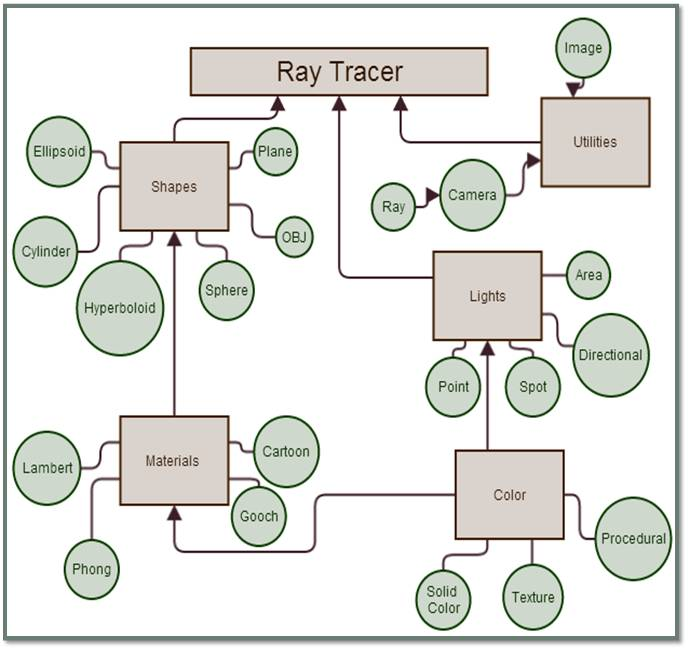
\includegraphics[height=3.0in]{figures/rayTracerStructure.jpg}
\caption{Diagram of the Parenting/Dependency Structure of the Ray Casting Program explained}
\label{fig:RayTracerDependencies}
\end{figure}
In order to successfully determine how classes should be established, it is important to plan how classes should relate to one another.  The relationships of each class to one another can most successfully be summarized as such in Figure \ref{fig:RayTracerDependencies2}.  The picture represents the 4 main object types, \textbf{Shapes}, \textbf{Materials}, \textbf{Color}, \textbf{Lights}. In summary, every \textbf{shape} must have a \textbf{material} which must have at least one \textbf{color}. A \textbf{shape} can be any of the circles sprouting locally around its pink square{sphere, ellipsoid, cylinder, etc..} just as a material can be any of the circles sprouting from it's pink square {Lambert, Phong, Cartoon}.  \textbf{Lights} do not have any connections with Shapes or materials, but each light must have a color.  Classes can be broken into two main elements, variables, which hold data within the class, and functions, which mold the data that is held within the class.  In all languages, variables have a specific type, for instance integers(whole numbers), floats(decimal numbers), and strings(words or letters).  Classes are a way to introduce new variable types.  If I were to create a Shape class, I could when make Shape variables that determine their properties from the Shape class.  The following is an abstract summary of each of the primary variables and functions for each Major Class type established in this raytracer.
\subsubsection{Shapes}
The Shape class consisted of 4 main variables and 3 main functions. Figure \ref{uml:shapeclass} Unified Modeling Language diagram demonstrates the class.

\begin{figure}[ht]

\centering
\includegraphics{class_diagram.1}
\caption{Unified Modeling Language Diagram displaying important Shape Class features}
\label{uml:shapeclass}
\end{figure}

As we can see the Shape Class has all the important base functionality for every shape object.  Associated with every shape object was a Vector that described it's position in 3d space, a Vector that was calculated to describe where a light ray or camera view ray would hit the shape (Hit Point), a Material Object that described what the shape would look like when interacting with the light and camera view vectors and a Distance integer that helped to sort all the shapes in the scene from closes to furthest away.  The shapes initially had 3 important base functions that calculated if the shape intersecting a light ray (intersect), what the return Color would be based off of the material on the object (rtnColor) and the Surface normal that was given from the intersection point (calcNormal).  These 3 functions were inherited to all the children shape objects.

\subsubsection{Color}
The Color parent object was a class that incorporated all types of color information that could be displayed in a Material.  The color objects were Vectors that held Red, Green, and Blue(RGB) hue information but could also be added and subtracted from one another.  Color information could also be taken from an image or a procedural equation to describe the RGB information transmitted from the surface. Figure \ref{uml:colorclass} shows the color class.

\begin{figure}[ht]
\centering
\includegraphics{class_diagram.3}
\caption{Unified Modeling Language Diagram displaying important Shape Class features}
\label{uml:colorclass}
\end{figure}

The color parent object held Color information in a Vector, and a method that described how to calculate the color vector.

\subsubsection{Materials}
The parent material class consisted of 2 components, as demonstrated in Figure \ref{uml:materialclass}.

\begin{figure}[!ht]
\centering
	\includegraphics{class_diagram.2}
\caption{Unified Modeling Language Diagram displaying important Shape Class features}
\label{uml:materialclass}
\end{figure}

As we can see the Material class very simply had a variable that stored a Color object, which described which color would be used when calculating the returned color from the returnColor function.  These variables were either overwritten or added onto in child classes but the base Material Parent class was used as a holder for all material objects.
\subsubsection{Lights}
A light object was very simple and followed the UML Diagram in Figure \ref{uml:lightclass}:
\begin{figure}[!ht]
\centering
	\includegraphics{class_diagram.4}
\caption{Unified Modeling Language Diagram displaying important Shape Class features}
\label{uml:lightclass}
\end{figure}
A parent light object only held the information needed to determine the color for the light so the variables were the Color Object and Position Vector and the function calculated if the light intersected with the object and if it did, what color would be returned from the light's Color object.

\subsection{Declaring Classes With each Language}
For this section we will use the Shape class to demonstrate how classes are declared in each language.  The Shape class structure is defined in figure \ref{uml:shapeclass}.
\subsubsection{C++}
%TODO: C++ Class Declaration
\begin{lstlisting}[language=C++, caption=C++ Class definition example, style=mystyle]
vector <Sphere> sphere_list;
Sphere sphere_object = new Sphere();
sphere_list.push_back(sphere_object);
\end{lstlisting}
\subsubsection{Using C++ classes}
%TODO: C++ class syntax
\subsubsection{Processing}
%TODO: Java Class Declaration
\begin{lstlisting}[language=Java, caption=Java Class definition example, style=mystyle]
ArrayList<Sphere> sphere_list = new ArrayList<Sphere>();
Sphere sphere_object = new Sphere();
sphere_list.add(sphere_object);
\end{lstlisting}
\subsubsection{Using Processing classes}
%TODO: Processing class syntax
\subsubsection{Python}
%TODO: Python Class Declaration
\begin{lstlisting}[language=Python, caption = Example of class definition in Python, style=mystyle]
//shape.py file//
class Shape(object):
    __init__(self,...):
        //shape constructor
    def size(self,...):
        //size calculation for all child classes
\end{lstlisting}
\subsubsection{Using Python classes}
%TODO: Python class syntax
\subsection{Dynamic Class Variables}
%TODO: Pass by reference within classes to introduce polymorphism
Since Processing and C++ are both strong-typed languages, eliminating the data type issue is not possible, but there is a solution.  Cardelli and Peter describe strong-typed, or static-typed, languages in their article entitled textit{On Understanding Types, Data Abstraction, and Polymorphism} as follows
\begin{quote}
Static typing allows type inconsistencies to be discovered at compile time and guarantees that executed programs are type-consistent. It facilitates early detection of type errors and allows greater execution-time efficiency. It enforces a programming discipline on the programmer that makes programs more structured and easier to read. \cite{cardelli1985understanding}
\end{quote}

Two computer science terms called \textit{inheritance} and \textit{polymorphism} will help to solve this problem.  Inheritance is the idea that a child class can inherit the properties and functions of a parent class.  Cardelli and Wegner also explain different types of polymorphism, and from their explanation the type used for this thesis is called subtyping.
\begin{quote}
Subtyping is an instance of \textit{inclusion polymorphism}. The idea of a type being a subtype of another type is useful not only for subranges of ordered types such as integers, but also for more complex structures
such as a type representing Toyotas which is a subtype of a more general type such as Vehicles. Every object of a subtype can be used in a supertype context in the sense that every Toyota is a vehicle and can be
operated on by all operations that are applicable to vehicles. \cite{cardelli1985understanding}
\end{quote}
To introduce how this is achieved in each language, the topic of ``pass-by-value" and ``pass-by-reference" must be discussed.  In both C++, when declaring an object, two variations can be done in relation to the memory organization within the computer.  The first, ``pass-by-value" is the most common and everytime a variable changes or moves, a \textit{copy} of the variable is made within the backend and saved in a new location.  However another schema exists, ``pass-by-reference", which rather than copies the data creates a reference or ``pointer" back to the original variable.
\subsection{Data Structures}
Accomplishing the data structure task in Python is the most simple and takes no extra effort.  Simply declare an object and place it in a Python list, like so:
\begin{lstlisting}[language=Python, caption=Python List Example, style=mystyle]
sphere = Sphere.Sphere();
cube = Cube.Cube();
objects =  [];
objects.append(sphere);
objects.append(cube);
\end{lstlisting}
That code will create a sphere object, cube object, and an objects list, and then add the sphere and cube into the data structure with the lists append method.  Python lists can accept any combination of different variable types, which can be useful for a ray-tracers implementation but dangerous for software prosperity and robustness.  If we are assuming that all variables in a list have the same type and therefore the same associated functions and an object that does not fall under these assumptions gets added to the list, this will cause the program to fail.  More care needs to be taken to make sure all variables are of the correct type that are added to a list to be sure that the program will run successfully, since this is not required for the program to start running in the first place.

That is the reason why it is more difficult to accomplish the data structure task in C++ and Processing(Java).  All objects must be of the same type to add them to a data structure.  Furthermore the most basic data structure, an Array, must be declared a specific size upon initialization.  The size issue can be easily circumvented however.  For each of these there is a dynamic container that will grow and shrink in size. C++ has a vector data structure and Processing has an ArrayList. To declare each is simple:
\begin{lstlisting}[language=C++, caption=C++ Vector Example, style=mystyle]
vector <Sphere> sphere_list;
Sphere sphere_object = new Sphere();
sphere_list.push_back(sphere_object);
\end{lstlisting}
\begin{lstlisting}[language=Java, caption=Java ArrayList Example, style=mystyle]
ArrayList<Sphere> sphere_list = new ArrayList<Sphere>();
Sphere sphere_object = new Sphere();
sphere_list.add(sphere_object);
\end{lstlisting}
Each of these examples creates a \textit{Sphere} list, an instance of a \textit{Sphere} object, and then puts that \textit{Sphere} object into the \textit{Sphere} list.  Note that each structure \textit{must} be declared as the type of object that is being placed into it.  Since Processing and C++ are both strong-typed languages, eliminating the data type issue is not possible, but there is a solution.  Cardelli and Peter describe strong-typed, or static-typed, languages in their article entitled textit{On Understanding Types, Data Abstraction, and Polymorphism} as follows
\begin{quote}
Static typing allows type inconsistencies to be discovered at compile time and guarantees that executed programs are type-consistent. It facilitates early detection of type errors and allows greater execution-time efficiency. It enforces a programming discipline on the programmer that makes programs more structured and easier to read. \cite{cardelli1985understanding}
\end{quote}

Two computer science terms called \textit{inheritance} and \textit{polymorphism} will help to solve this problem.  Inheritance is the idea that a child class can inherit the properties and functions of a parent class.  Cardelli and Wegner also explain different types of polymorphism, and from their explanation the type used for this thesis is called subtyping.
\begin{quote}
Subtyping is an instance of \textit{inclusion polymorphism}. The idea of a type being a subtype of another type is useful not only for subranges of ordered types such as integers, but also for more complex structures
such as a type representing Toyotas which is a subtype of a more general type such as Vehicles. Every object of a subtype can be used in a supertype context in the sense that every Toyota is a vehicle and can be
operated on by all operations that are applicable to vehicles. \cite{cardelli1985understanding}
\end{quote}
Subtyping will allow us to accomplish the example that if both a sphere class and a cube class need a move function that will reposition it within the scene, a parent Shape class can be established that will provide inherited logic for each class.  If each object also needed a resize class, but the sphere needed to resize differently than all other objects, the size function can also be rewritten in the sphere class.  The type Shape can be subtyped in to Sphere and Cube to accomplish shape specific logic as needed.  This is accomplished in C++ as follows:

\singlespacing
\begin{lstlisting}[language=C++, style=mystyle]
//shape.h file//
class Shape
{
    public:
        Shape(){};
        float move(){
            //calculate size for all objects
        }
        virtual float size(){
            //calculate size for all objects
        }
}
\end{lstlisting}
\begin{lstlisting}[language=C++, style=mystyle]
//sphere.h file//
#include "shape.h"
class Sphere: public Shape
{
    public:
        Sphere(){};
        float size(){
            //calculate sphere size logic.
        }
}
\end{lstlisting}
\begin{lstlisting}[language=C++, caption=C++ Inheritance Example, style=mystyle]
//cube.h file//
#include "shape.h"
class Cube: public Shape
{
    public:
        Cube(){};
}
\end{lstlisting}
\doublespacing
In the above example, all classes will have a move function and a size function, but the size function for the Sphere class will function differently than the size function for the Shape/Cube class because it has been overwritten.  All children classes need to call their own constructors in order to be instantiated.  It is important to note that a child class must contain ``\#include `sphere.h'" or else it will not work correctly. In order to rewrite a parent function in a child class, the keyword virtual needs to be used as seen on the size function in the shape.h example.  To accomplish this same procedure in Processing, classes need to be established as follows:

\singlespacing
\begin{lstlisting}[language=Java, style=mystyle]
//shape.pde file//
abstract class Shape
{
    Shape(){};  //Constructor
    float size(){
        //calculate size for all object types;
    }
}
\end{lstlisting}
\begin{lstlisting}[language=Java, caption=Java Abstract Class Example, style=mystyle]
\label{listing:Java Abstract Class Example}
//sphere.pde file//
class Sphere extends Shape
{
    Sphere(){};
    float size(){
        //calculate size specific for sphere
    {
}
\end{lstlisting}
\doublespacing
The syntax for the cube.pde file is the same as the sphere.pde with the extends keyword showing that the sphere is the child of the Shape class.
\begin{center}
\line(1,0){100}
\end{center}
\subparagraph{Note:Python Classes}
While parent classes are not important for Python list functionality because Python can be considered a dynamic type language (as opposed to the static type for C++ and Java), for organizational purposes they were used and inheritance was declared as follows (note tabs and spacing), using the same example:
\singlespacing
\begin{lstlisting}[language=Python, style=mystyle]
//shape.py file//
class Shape(object):
    __init__(self,...):
        //shape constructor
    def size(self,...):
        //size calculation for all child classes
\end{lstlisting}
\begin{lstlisting}[language=Python, caption=Python Class Inheritance Example, style=mystyle]
//sphere.py file//
import Shape
class Sphere(Shape.Shape):
    def __init__(self,...):
        //sphere constructor contents
    def size():
        //calculate size specific for sphere
\end{lstlisting}
\begin{center}
\line(1,0){100}
\end{center}
\doublespacing
\paragraph{} Now that the class structure has been established for each strict-type language to promote a single object data container, which will mirror the ray tracing structure theory, establishing the data structure for each language needs to be adjusted.  The ``pass-by-reference" tactic in C++ is what will allow different variable types to be saved to a common parent data structure, as follows:
\begin{lstlisting}[language=C++, caption=C++ Vector Example, style=mystyle]
vector <Shape*> shape_list;
Sphere *sphere_object = new Sphere();
sphere_list->push_back(sphere_object);
\end{lstlisting}
Declaring the vector with the ``*" denotes a C++ pointer, or that the variable will use the pass-by-reference schema.  Pass-by-reference and pass-by-value variables cannot be combined within a data structure.  To then call any functions within the pointer variables, you must use ``->" rather than ``.".  This allows us to save all different shape objects within the same data structure.  To accomplish this is Processing you may have noticed that in \ref{listing:Java Abstract Class Example} that the Shape class was declared as Abstract.  This keyword signifies that an object of this type may not be instantiated within a program.  This keyword demonstrates true inheritance because it acts as a placeholder for commonly used functions and variables between class types.  In Java, it will allow us to declare child classes as common types without losing each classes individual functions and variables. This is accomplished as follows:
\begin{lstlisting}[language=Java, caption=Java ArrayList Example, style=mystyle]
ArrayList<Shape> shape_list = new ArrayList<Shape>();
Shape sphere_object = new Sphere();
Shape cube_object = new Cube();
shape_list.add(sphere_object);
shape_list.add(cube_object);
\end{lstlisting}
\doublespacing
Notice that we are declaring sphere\_object and cube\_object as a type Sphere but using the child classes individual constructors.  This will allow us to call ``shape\_list.add()" on the next two lines without throwing an error.  If the Shape class was not declared as abstract, when declaring Shape sphere\_object and calling the child constructor, and functions that are specific to the child class will be replaced with the parent classes functions.  While Java still has ``pass-by-value" and ``pass-by-reference", Processing/Java has simplified their language to effectively made all declared variables function as pointers, pointing back to the original variables declaration.

\subsection{Milestone Results: Processing Time Overview and Images}
Once the issues with Class and Object declaration were solved, implementing the Basic Ray Casting Milestone was very straight forward with each language.  However there was one issue with the processing language that accounted for a majority of the Processing implementation, and accounts for a core theory of ray tracing implementation.
\subsubsection{Left Hand vs. Right Hand Rule}
In the 3-D virtual world, there is a set of governing rules that determine an objects position within the space, known as a coordinate plane.  Just like on a two dimensional graph there is an X and Y coordinate, in a 3-D scene there is a new coordinate Z added.  The order and direction for each of these axis, as they're called, determines many important calculations when determining size and space of objects in the scene.  Left-handed and right handed can be described as follows:

\begin{quote}
In order to draw something at a point in three dimensions the coordinates are specified in the order you would expect: x, y, z. Cartesian 3D systems are often described as "left-handed" or "right-handed." If you point your index finger in the positive y direction (up) and your thumb in the positive x direction (to the right), the rest of your fingers will point towards the positive z direction. It's left-handed if you use your left hand and do the same.
\end{quote}
For the C++ and Python implementations of the ray tracers, a coordinate system needed to be created from scratch, and since the researcher is right handed a right handed, a right handed coordinate system was used.  This means, when looking at a computer monitor, the positive y axis pointed towards the top of the screen, the positive X axis pointed to the right of the screen and the Z axis points directly out of the screen, perpendicular to the screens surface.  However, this is not typically a traditional schema for coordinate planes with computers, nor was it the scheme used by Processing.  Processing used a left-handed coordinate system where the positive y axis points towards the bottom of the screen, the positive x axis points towards the right of the screen, and the positive z points away from the user, towards the back of the computer, perpendicular with the computer screen.  Many of the calculations associated with cross products and other Vector Math needed to have the y value and z value negated so that it behaved more similarly to the other two ray tracing programs
\subsection{Basic Ray Casting Images}
Here are a few Image from the Basic Ray Casting Milestone.  While these are just a few examples from each language and each task, each language accomplished the same types of images that are presented.
\begin{figure}[ht]
\centering
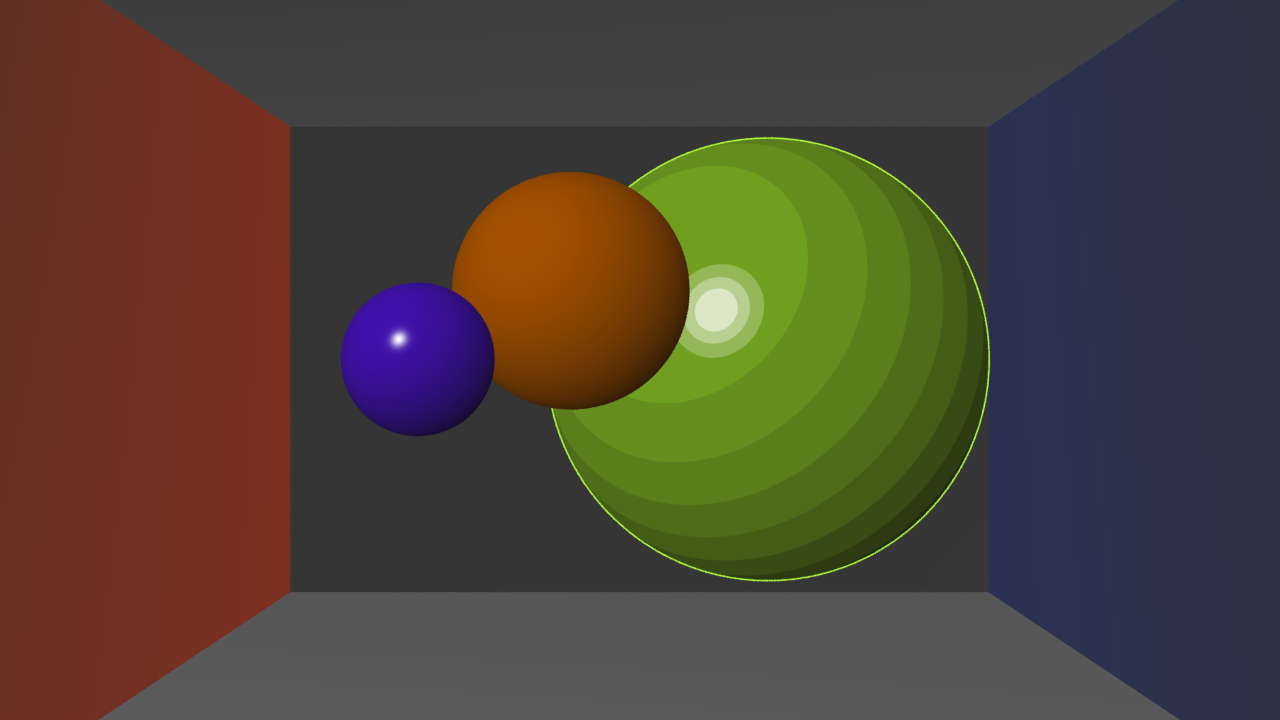
\includegraphics[width=\textwidth]{figures/BasicRayCastingProcessing.png}
\caption{Ray Casting Accomplished with Processing. Shown are three spheres with a different texture type for each, and five planes all with flat textures applied.}
\label{fig:processingraycasting}
\end{figure}

\begin{figure}[ht]
\centering
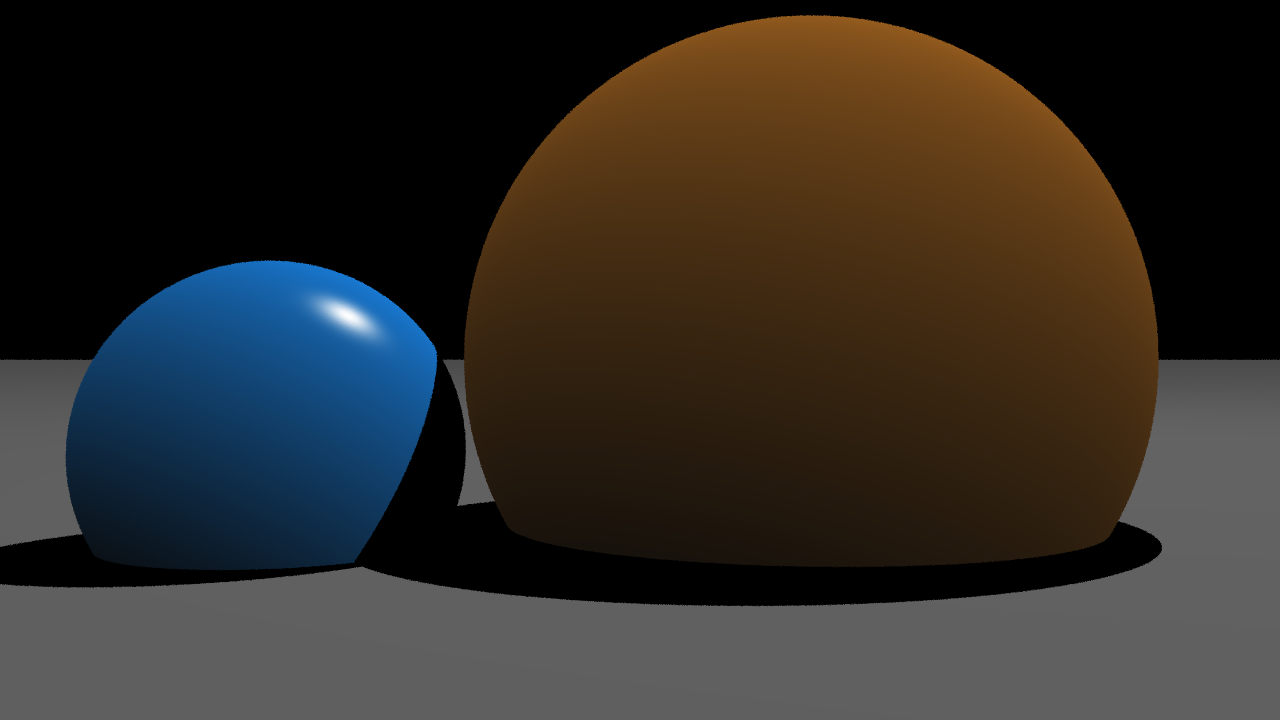
\includegraphics[width=\textwidth]{figures/ShadowCastingPython.png}
\caption{Ray Casting Accomplished with Python.  Shown are two spheres, and one plane that all cast shadows from a simple point light. }
\label{fig:pythonraycasting}
\end{figure}

\begin{figure}[ht]
\centering
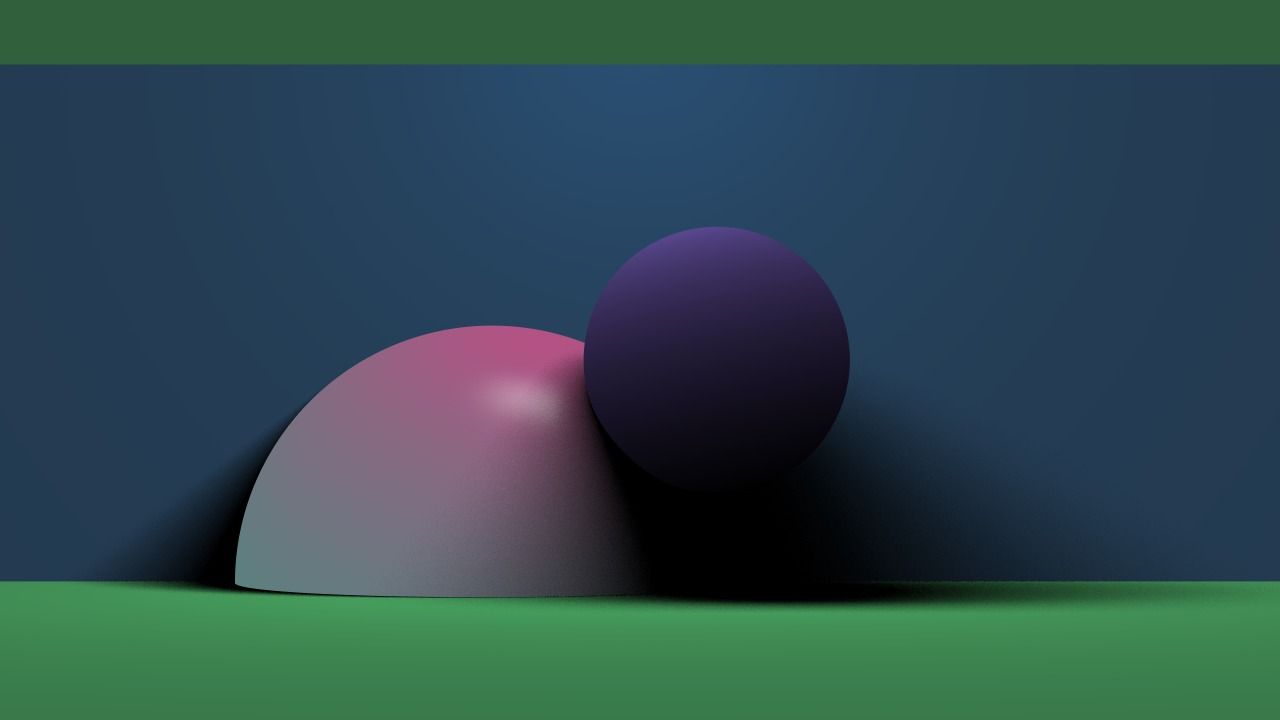
\includegraphics[width=\textwidth]{figures/ShadowCastingC++.jpeg}
\caption{Ray Casting Accomplished with C++.  Shown are two spheres, five planes and an area light that all cast shadows, which accounts for the soft shadow effect. }
\label{fig:cplusraycasting}
\end{figure}

\begin{figure}[ht]
\centering
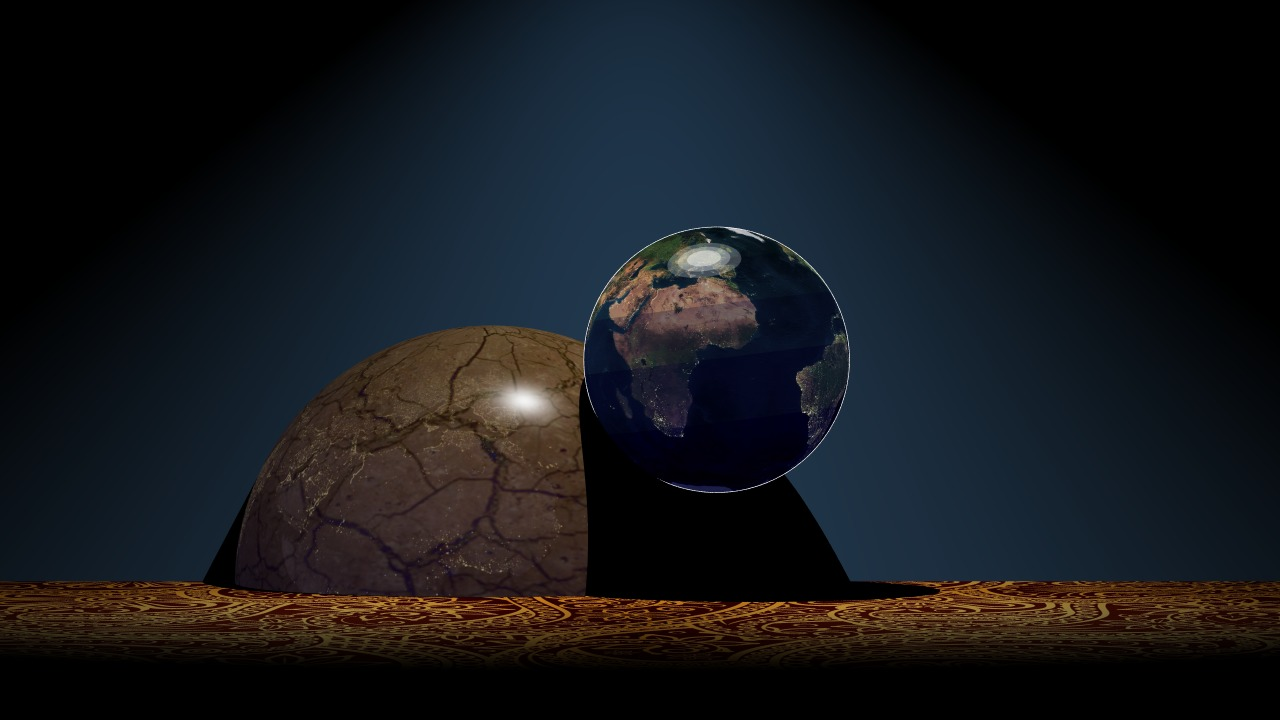
\includegraphics[width=\textwidth]{figures/texturingC++.jpg}
\caption{Ray Casting Accomplished with C++.  Shown are two spheres with 2 separate shader types with two separate images mapped to them, and two planes, one with a repeated image texture and one without any image texture. }
\label{fig:cplusraycasting}
\end{figure}

\begin{figure}[ht]
\centering
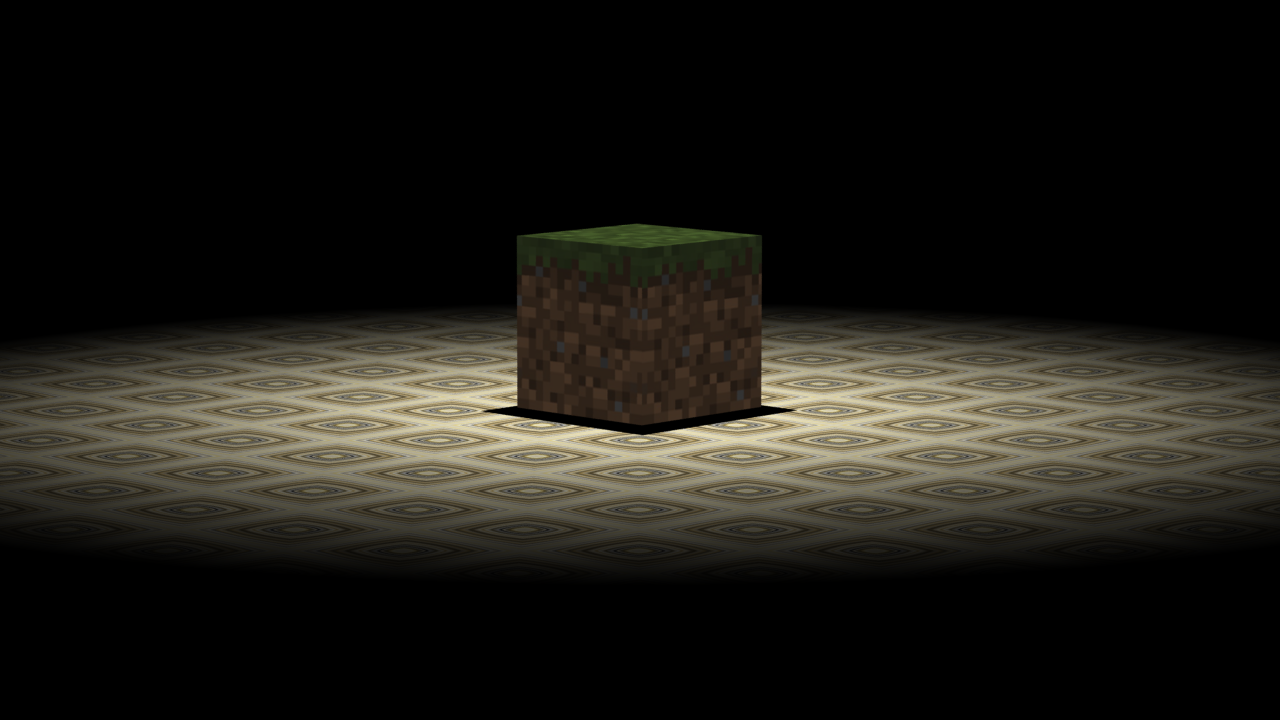
\includegraphics[width=\textwidth]{figures/processingTriangles.png}
\caption{Ray Casting Accomplished with Processing. One cube with twelve triangles and an image mapped to it on a plane with a repeated image texture illuminated by a spotlight.}
\label{fig:processingtriangles}
\end{figure}

\subsection{Performance Results}
For each test in Basic Ray Casting, a variety of levels of complexity were tested in order to see how each language can process a different amount of load.  For each rendering a 1280 x 720 image size was used to generate a high quality image for testing.  The results are graphed and labeled as follows:
\begin{figure}[ht]
\centering
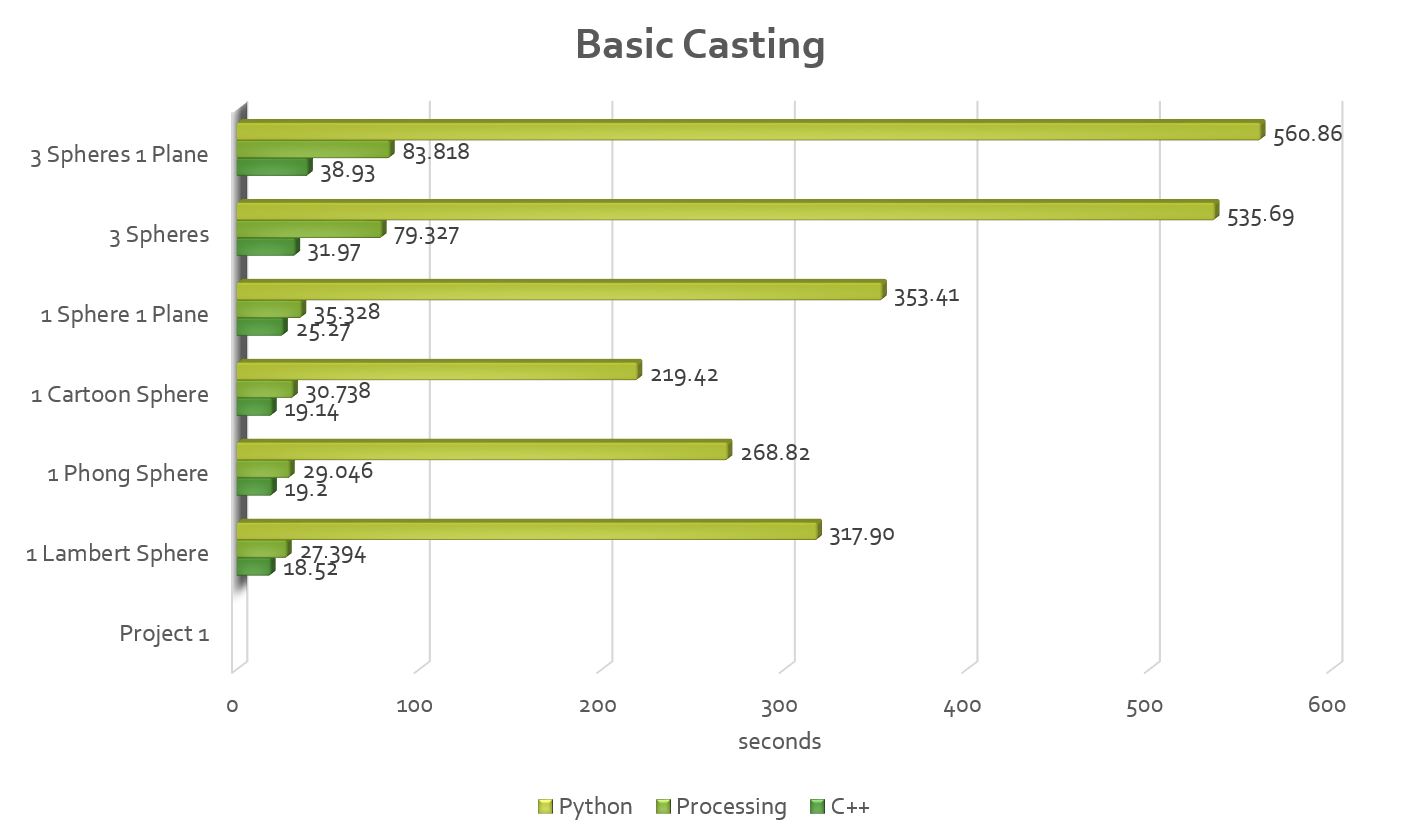
\includegraphics[width=\textwidth]{figures/graphs/basic-graph.png}
\caption{Basic Performance Graph filler}
\label{fig:basicgraph}
\end{figure}

\begin{figure}[ht]
\centering
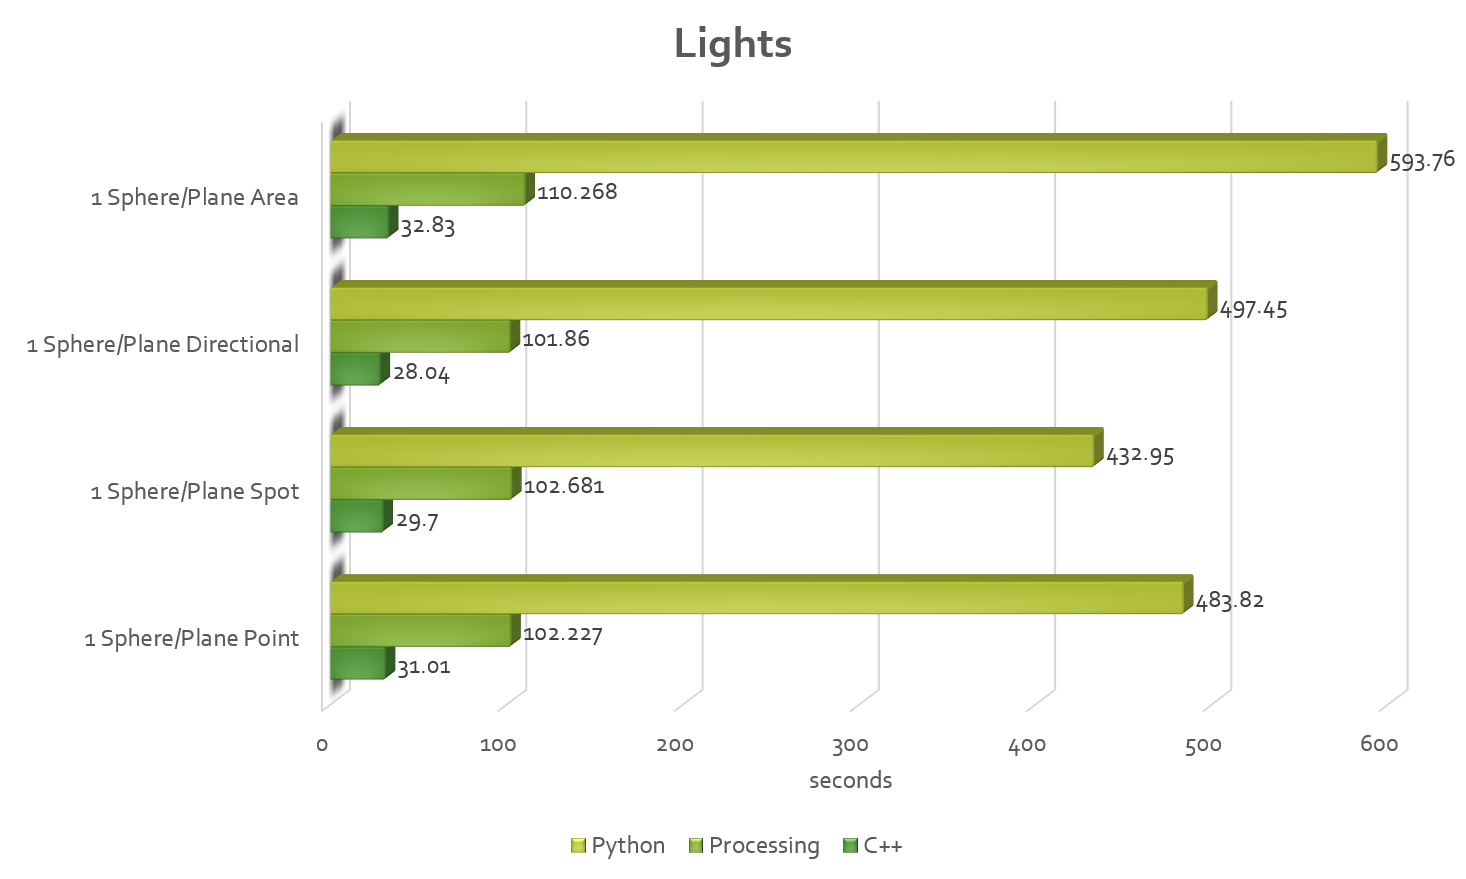
\includegraphics[width=\textwidth]{figures/graphs/lights-graph.png}
\caption{Basic Performance Graph filler}
\label{fig:lightsgraph}
\end{figure}

\begin{figure}[ht]
\centering
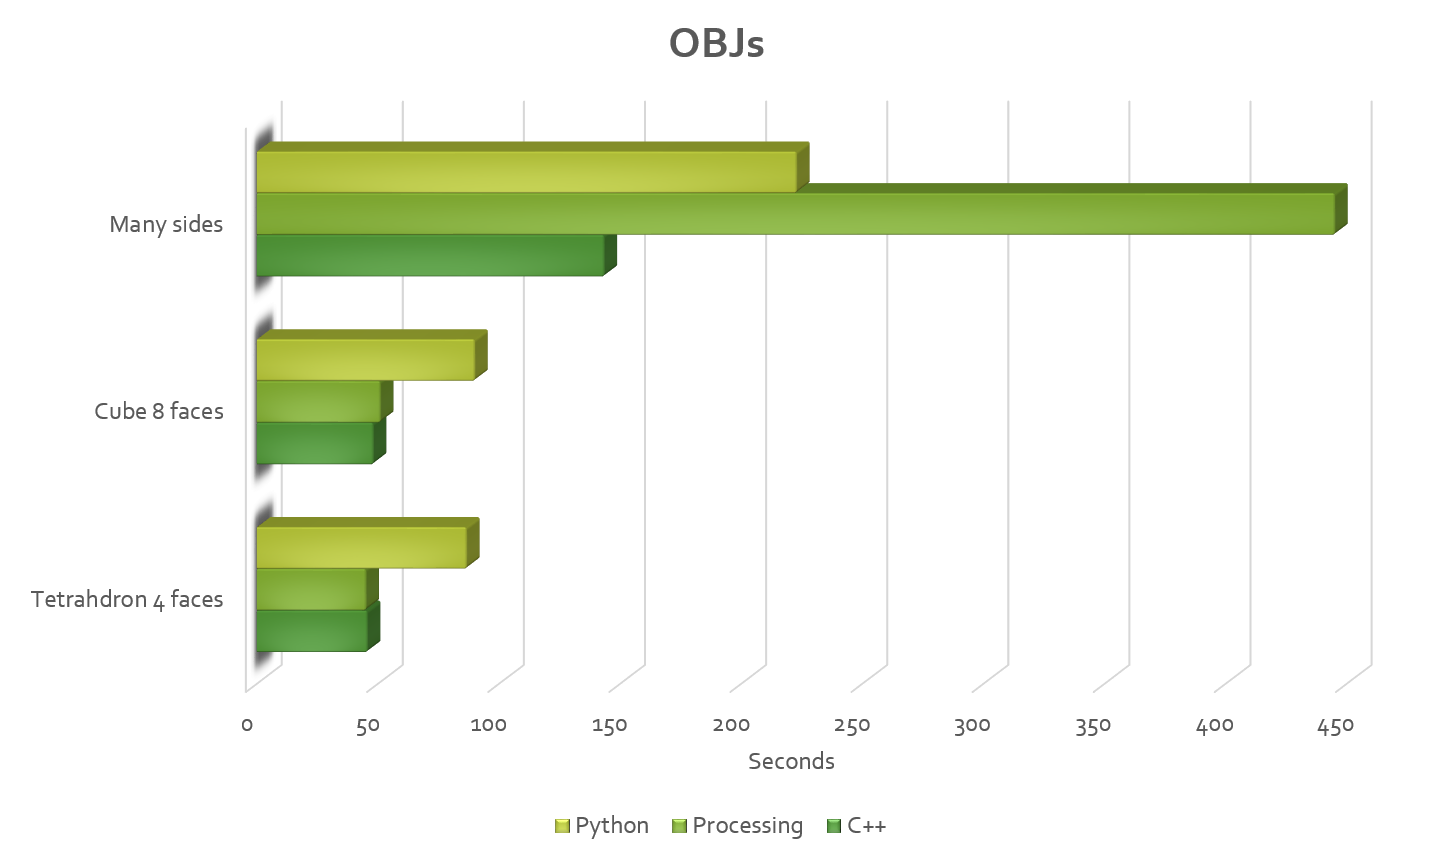
\includegraphics[width=\textwidth]{figures/graphs/obj-graph.png}
\caption{Basic Performance Graph filler}
\label{fig:basicgraph}
\end{figure}

\begin{figure}[ht]
\centering
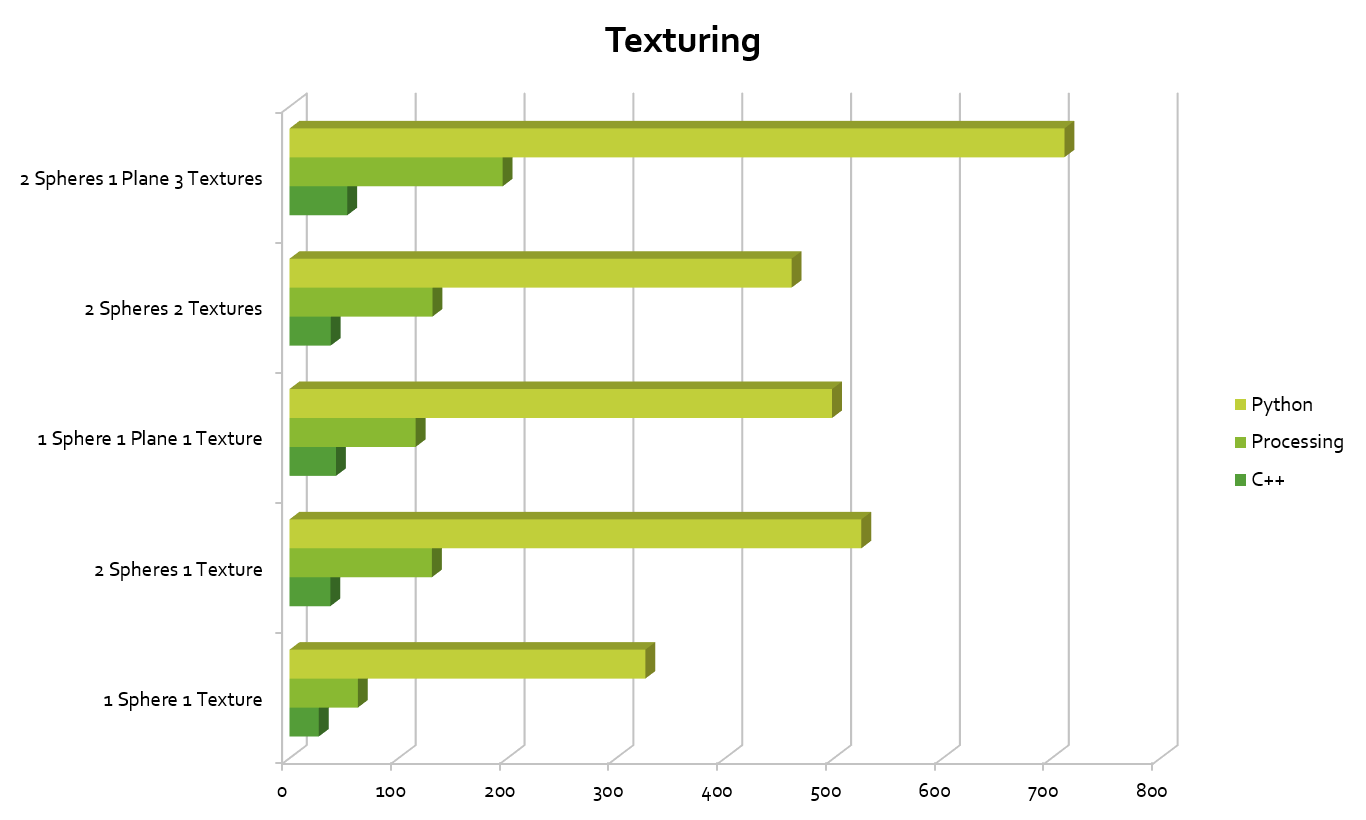
\includegraphics[width=\textwidth]{figures/graphs/texturing.png}
\caption{Basic Performance Graph filler}
\label{fig:basicgraph}
\end{figure}

%%%%%%%%%%%%%%%%%%%%%%%%%%%%%%%%%%%%%%%%%%%%%%%%%%%%%%
%%%%%%%%%%%%%%%%%%%%%%%%%%%%%%%%%%%%%%%%%%%%%%%%%%%%%%
\section{Milestone 3: Ray Tracing and Distributed Ray Tracing}
The main complications discovered for this milestone where all related to the implementation of a recursive ray tracing strategy.  All three languages had the same difficulties that were not unique to each implementation.  To implement recursion requires the knowledge of establishing a process function within each raytracing function that will repeatedly call itself unless specific escape conditions are met.  It is important to establish these conditions such that they are met within the execution of the program or else the ray tracer will implement an infinite loop that will consume computing resources until the computer crashes and needs to be restarted.  

\subsection{Basic Ray Casting Images}
Very Beautiful
\subsection{Performance Results}
So fast

\section{Milestone 4: Indirect Illumination}
Milestone 4 established the same complications that Milestone 3 had, with the majority of the implementation being the same throughout all three languages.
\subsection{Basic Ray Casting Images}
Very Beautiful
\subsection{Performance Results}
So fast
